%% Supplementary information for the optimization manuscript (main.tex).
%% Tables are generated by analysis/opt_stats.py and analysis/si_tables.py from the
%% dose records in data/; rebuild them before this file.
\documentclass[11pt]{article}
\usepackage[T1]{fontenc}
\usepackage{lmodern}
\usepackage[margin=2cm]{geometry}
\usepackage{amsmath}
\usepackage{graphicx}
\usepackage{booktabs}
\usepackage{longtable}
\usepackage{tabularx}
\usepackage[per-mode=symbol]{siunitx}
\usepackage[dvipsnames]{xcolor}
\usepackage[hidelinks]{hyperref}
\usepackage{caption}
\usepackage{microtype}
\renewcommand{\thetable}{S\arabic{table}}
\renewcommand{\thefigure}{S\arabic{figure}}
\renewcommand{\thesection}{S\arabic{section}}
\newcommand{\ph}[1]{\textcolor{orange!75!black}{\textsf{[#1]}}}
\captionsetup{font=small}
% \input is not expandable inside tabulars; the primitive is
\makeatletter\newcommand{\tabinput}[1]{\@@input #1 }\makeatother

\title{Supplementary information for\\[4pt]
\large Per-powder Bayesian calibration of an auger doser for alloy feedstock preparation, and dosing records as a probe of powder flow}
\author{Will Mulberry, Sam Charles, Luke Winters, Carl Robison, Gage Erickson, Sterling G. Baird}
\date{}

\begin{document}
\maketitle

\noindent Every table here is generated from the dose records in the repository
(\url{https://github.com/vertical-cloud-lab/powder-doser}, directory \texttt{paper/optimization}):
\texttt{data/opt\_trials/} holds the 125 records (MongoDB collection \texttt{opt\_trials}, 29 September
to 20 October 2026), and \texttt{analysis/opt\_stats.py}, \texttt{analysis/gp\_diagnostics.py} and
\texttt{analysis/si\_tables.py} compute every number in the main text and these tables. Settings are
abbreviated as: taps bulk/trickle, bulk tilt ($^\circ$), trickle tilt ($^\circ$), tap tilt ($^\circ$),
bulk speed (rpm), switch threshold (g to go), stopping band $\delta$ (mg).

\section{Campaign 1 and its validation (salt, target 0.5~g)}

\begin{table}[h]
\centering
\caption{Screening main effects of campaign~1, from its 16 corners (eight at each level of every setting).
Time is averaged over the corners that ended inside their band (number in brackets), because an overshoot
ends in seconds and would look fast; $|e|$ is averaged over all eight; ``fails'' counts overshoots and jams.}
\label{tab:maineffects}
\small
\begin{tabular}{@{}llrrrrrr@{}}
\toprule
 & Levels & \multicolumn{2}{c}{Time of ok doses (s)} & \multicolumn{2}{c}{Mean $|e|$ (mg)} & \multicolumn{2}{c}{Fails} \\
Setting & low / high & low & high & low & high & low & high \\
\midrule
\tabinput{analysis/results/tables/si_main_effects.tex}
\bottomrule
\end{tabular}
\end{table}

\scriptsize\setlength{\tabcolsep}{3.2pt}
\begin{longtable}{@{}rlllllllllrrr@{}}
\caption{Every dose of campaign~1 (indices 0--41, 29 September 2026) and of the two validation blocks
(indices 42--59, 6 October 2026). Doses 42 and 43 ran at the recommended settings before a restart of the
rig and belong to neither block; 44--51 are the \texttt{bo-005} block and 52--59 the \texttt{corner-09}
block. Error is signed (negative: under the target). Outcome is the controller's classification when it
stopped; the error is scored on the settled reading 2~s later, so a dose can be ``ok'' and settle just outside
its band (dose 20: $-$9.5~mg at $\pm$9~mg). Feed: mass gained between the first and last reading of the bulk
stage divided by its duration (mg/s; ``--'' where the bulk stage lasted under 3~s or has no telemetry), the
quantity behind Fig.~3b and the paired-corner statistics of Section~3.2.}\label{tab:salt}\\
\toprule
\# & Label & Taps & Bulk & Trickle & Tap & rpm & Switch & $\delta$ & Outcome & $t$ (s) & $e$ (mg) & Feed \\
\midrule
\endfirsthead
\toprule
\# & Label & Taps & Bulk & Trickle & Tap & rpm & Switch & $\delta$ & Outcome & $t$ (s) & $e$ (mg) & Feed \\
\midrule
\endhead
\tabinput{analysis/results/tables/si_salt_doses.tex}
\bottomrule
\end{longtable}

\begin{table}[h]
\centering
\caption{Single doses of salt at the recommended settings (\texttt{bo-005}) with targets from 5~mg to 10~g
(6 and 8 October 2026). The 10~g dose finished, then ended with a firmware fault while it reported; its mass
is from the console log.}
\label{tab:range}
\small
\begin{tabular}{@{}lrlrrr@{}}
\toprule
Started (UTC) & Target (g) & Outcome & $t$ (s) & $e$ (mg) & Taps \\
\midrule
\tabinput{analysis/results/tables/si_production_salt.tex}
\bottomrule
\end{tabular}
\end{table}

\section{Campaign 2 (salt, nine settings)}

\scriptsize\setlength{\tabcolsep}{3.2pt}
\begin{longtable}{@{}rllllllllrlrrr@{}}
\caption{Every dose of campaign~2 (13 and 15 October 2026); ``Margin'' is the hand-over margin of the
trickle stage. \texttt{not-tared}: the balance had not been tared, nothing was dispensed;
\texttt{fw-error}: the dose finished but the firmware ran out of memory while reporting it (fixed on 15
October, from dose 33). As in Table~\ref{tab:salt}, outcome is the controller's classification and the
error is scored 2~s later (dose 5: $-$3.1~mg at $\pm$3~mg). Feed as in Table~\ref{tab:salt}.}\label{tab:margin}\\
\toprule
\# & Label & Taps & Bulk & Trickle & Tap & rpm & Switch & $\delta$ & Margin & Outcome & $t$ (s) & $e$ (mg) & Feed \\
\midrule
\endfirsthead
\toprule
\# & Label & Taps & Bulk & Trickle & Tap & rpm & Switch & $\delta$ & Margin & Outcome & $t$ (s) & $e$ (mg) & Feed \\
\midrule
\endhead
\tabinput{analysis/results/tables/si_margin_doses.tex}
\bottomrule
\end{longtable}

\section{Metal feedstock}

\begin{table}[h]
\centering
\caption{Every executor dose and hand-driven session of metal feedstock (29 September to 20 October 2026).
Target is the mass that dose was asked for; hand-driven sessions (\texttt{manual}) were reverse turns,
read-backs and stepwise top-ups. Bulk feed, ``mean'': the mass gained between the first and last reading of
the bulk stage divided by its duration; ``middle'': the least-squares slope over the middle 60\% of the bulk
stage, which leaves out the start-up and the end-of-stage taper. The two differ most for short or tapering
stages (the last Al~4047 dose: 30.7 against 17.9~mg/s; 22.9~mg/s over the whole dose). In the bulk-only mode
of the Al~4047 doses the auger slowed linearly over the last 0.1--0.5~g and sped up again after 3~s without
flow, so the bulk settings were nominal. The dose of 30 September at 21:21 ran 803~s (369~s of bulk, then 240 tap
cycles) before it ended at its tap-cycle budget; its executed parameters do not include the 600~s timeout of
the campaign doses. The charges these doses filled are reported with
the hardware (Charles et al.).}
\label{tab:metal}
\small
\begin{tabular}{@{}llllrrrr@{}}
\toprule
 & & & & & & \multicolumn{2}{c}{Bulk feed (mg/s)} \\
Started (UTC) & Powder & Mode & Target (g) & Outcome & $t$ (s) & mean & middle \\
\midrule
\tabinput{analysis/results/tables/si_metal_doses.tex}
\bottomrule
\end{tabular}
\end{table}

\section{Checks of the campaign's model (machine-learning checklist)}

\begin{table}[h]
\centering
\caption{Leave-one-out cross-validation on the 42 doses of campaign~1, with the outcomes encoded as the
campaign encoded them (jams at the 180~s / 20~mg limits or their true value if worse; overshoots at their
measured values). $\rho$: Spearman correlation of prediction and observation ($p$ in brackets; not defined
for the constant model). RMSE: root-mean-square error. Coverage: share of held-out doses inside the
95\% predictive interval (including dose-to-dose noise). $z$ SD: standard deviation of the standardized
residuals (1 if the uncertainty is right). Shapiro: $p$ of the Shapiro--Wilk test on those residuals.}
\label{tab:gpcv}
\small
\begin{tabular}{@{}llrrrrr@{}}
\toprule
Objective & Model & $\rho$ ($p$) & RMSE & Coverage (\%) & $z$ SD & Shapiro $p$ \\
\midrule
\tabinput{analysis/results/tables/si_gp_cv.tex}
\bottomrule
\end{tabular}
\end{table}

\begin{table}[h]
\centering
\caption{Relevance of each setting in the SAAS GP refitted on all 42 doses: median over the posterior draws of
the inverse length scale (larger means the objective changes faster with that setting).}
\label{tab:relevance}
\small
\begin{tabular}{@{}lrrrrrrrr@{}}
\toprule
 & Bulk taps & Trickle taps & Bulk tilt & Trickle tilt & Tap tilt & Bulk rpm & Switch & $\delta$ \\
\midrule
\tabinput{analysis/results/tables/si_gp_relevance.tex}
\bottomrule
\end{tabular}
\end{table}

\begin{figure}[h]
\centering
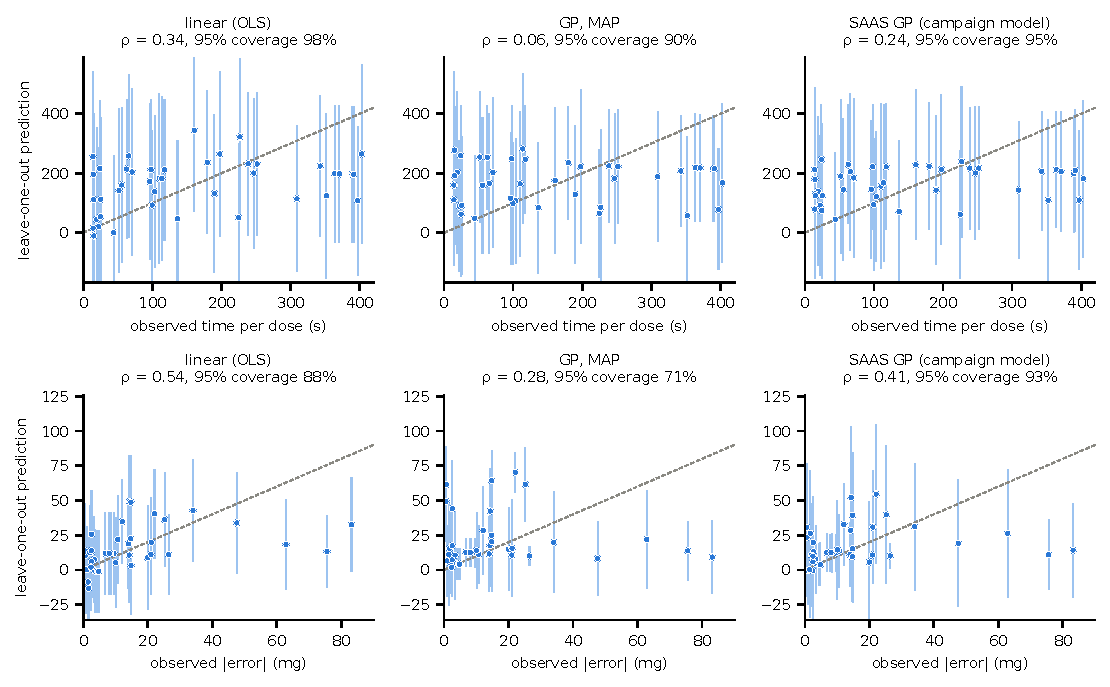
\includegraphics[width=\textwidth]{figures/figS_gp_cv}
\caption{Leave-one-out predictions (mean and 95\% predictive interval) against the observed time and
absolute error of the 42 doses of campaign~1, for the linear model, a standard GP fitted by maximum a
posteriori, and the campaign's SAAS GP.}
\label{fig:gpcv}
\end{figure}

\begin{table}[p]
\centering
\caption{How the manuscript addresses each item of Elsevier's machine-learning requirements for
\emph{Additive Manufacturing}. Two statistical models are essential to the conclusions: the SAAS GP of
the calibration campaigns, and the Spearman correlations of Section~3.6. The planned multi-task GP and
the DEM emulator will be added to this table when their results exist.}
\label{tab:mlrubric}
\small
\begin{tabularx}{\textwidth}{@{}p{3.6cm}X@{}}
\toprule
Item & Where and how \\
\midrule
1. Several models & The SAAS GP (one per objective) chooses doses and recommends settings; Spearman rank correlations test property links; a linear model, a MAP GP and a constant serve as baselines (Table~\ref{tab:gpcv}). \\
2. Model formulation & Purpose: sequential design and prediction (regression). Factors: eight settings (Table~2 of the main text), two categorical; responses: time per dose and absolute error; co-factors not modelled: day, fill state of the tube, humidity (their effect is shown in Section~3.2). Supervised. \\
3. Dataset & 42 doses of campaign~1 (Table~\ref{tab:salt}) and 43 of campaign~2 (Table~\ref{tab:margin}); the snapshot of all records and the scripts are public. Outcome encoding of failed doses is stated in Section~2.4. \\
4. Data support modelling & Screening corners give a balanced design (Table~\ref{tab:maineffects}); main effects are large compared with the scatter at the centre point for the error, not for time. Campaign~2 violates the assumption of a stationary response (Section~3.2), which is why its BO doses are not used for conclusions. \\
5. Is ML necessary? & Not shown at this sample size: a linear model ranks held-out doses as well as the GP (Table~\ref{tab:gpcv}). The GP is used for its calibrated predictive uncertainty, which the acquisition function needs; the recommendation it made held up in eight repeats. \\
6. Choice of model & SAAS prior because 8 settings and fewer than 50 doses; samples per parameter: 42 doses for a GP with 8 length scales, an outcome scale and a noise term per objective. \\
7. Training and testing & Leave-one-out cross-validation (Table~\ref{tab:gpcv}, Fig.~\ref{fig:gpcv}); NUTS with 256 warm-up and 128 retained draws (thinning 16); hyperparameter posteriors summarized in Table~\ref{tab:relevance}. Versions: Ax~0.4.3 for the campaign, BoTorch~0.18 for the checks. \\
8. Prediction performance & RMSE, rank correlation, interval coverage, standardized residuals and their normality (Table~\ref{tab:gpcv}); residuals of the error objective are heavy-tailed (overshoots), which no model captures; the validation block of the recommended settings fell inside the 95\% predictive intervals. \\
9. Impact & Against hand tuning (the prior practice): 3.1 times faster (2.7 at matched afterflow constant), exact $p = 0.004$; against picking the best observed dose: more accurate, $p = 0.005$ (Section~3.1). \ph{Multi-task benchmark against Sobol, single-task and carry-over baselines to be added.} \\
\bottomrule
\end{tabularx}
\end{table}

\section{Powder properties used in the correlations}

\begin{table}[h]
\centering
\caption{Literature and supplier values for the material class of the 12 powders whose fixed-setting
records (Charles et al.) enter Fig.~7. None was measured on the lots that were dosed. Provenance of the
Hausner ratio: \texttt{measured-product} (measured on the same commercial product),
\texttt{measured-class} or \texttt{measured-analog} (measured on the material class or a close analogue),
\texttt{class-band} (a typical range for the class), \texttt{aor-anchored-band} (a band chosen to agree
with the angle of repose), and \texttt{assumed-circular} (the tapped density was estimated from an assumed
Hausner ratio, so that ratio carries no independent information). Full sources: \texttt{data/powders/} and
\texttt{literature\_powder\_properties\_long.csv} on the branch named in \texttt{data/README.md}.}
\label{tab:props}
\footnotesize\setlength{\tabcolsep}{4pt}
\begin{tabular}{@{}lrrrrrrl@{}}
\toprule
Powder & Bulk (g/mL) & Tapped (g/mL) & Hausner & $d_{50}$ (\si{\micro\metre}) & AoR ($^\circ$) & Moisture (wt\%) & Provenance \\
\midrule
\tabinput{analysis/results/tables/si_properties.tex}
\bottomrule
\end{tabular}
\end{table}

\end{document}
